% !TeX spellcheck = en_US

Das ist die Methode.

\section{Task and requirements}

In Application, samples (for example cells) are frozen inside a thin ice layer. The sample can be stained with fluorescence and observed with cryo light microscopy. Also a sample can be prepared to study with cryo-transmission electron microscopy (cryo-TEM) . This allows to see samples in an hydrated state. This is only possible in cryo-TEM, as liquid water would evaporate in vaccuum \cite{Danino.2012}.

For sample preparation in cryo light microscopy and cryo-TEM, plunge-freezing is used \cite{Danino.2012} \cite{Faoro.2018}. This can be done either by hand or with a plunge-freezer, but both methods use the same steps. First, the slide is held by tweezers. then a 2 to 4 ml water drop including the sample is pipetted on the hydrophilic slide. Therefore the droplet spreads over the slide. Then the water droplet is blotted with filter paper, creating a thin film of water which is evaporating quickly. Then the slide is shot in cold liquid under -140°C, for example liquid ethane. A temperature drop of over 100°C freezes the water into a thin ice layer. With this procedure, vitificated ice is formed without a crystal structure.

A vitrificated sample is needed as ice crystals damage the samples and can disturb cryo light microscopy. Vitrificated ice is created by freezing water abruptly into temperatures under -120°C \cite{Wowk.2010}. To create a vitrificated sample, the slide needs a high thermal conductivity to freeze the water quickly. Also the liquid which is used to freeze the sample should not possess the Leidenfrost effect. The vapors which are created with the leidenfrost effect will prevent a rapid temperature drop. As liquid nitrogen has the leidenfrost effect, other liquids like liquid ethane are used.

The motivation for this master thesis is to find a way to use cryo light microscopy and cryo-TEM on the same sample. But currently, no slide is found which has all requirements to be used in plunge-freezing, cryo light microscopy and cryo-TEM. in plunge-freezing, a hydrophile surface is needed to archieve a thin ice layer. Additionally the thermal conductivity of the slide needs to be high for the steep temperature drop needed to create vitificed ice. For light microscopy, a transparent slide is not always required. But a good thermal conductivity is advantageous as less energy is needed to keep the sample cool (WAS FÜR VORRAUSSETZUNGEN GIBT ES DA?). In cryo-TEM, the sample needs to be extremely thin and small. Additionally, only light elements should be used as heavier electrons are disturbing the image in cryo-TEM.

To perform cryo-light microscopy and cryo-TEM, a sample transfer from one slide to another slide is proposed. The slide change must be performed at -140°C to maintain the vitrificated state of the sample. Additionally as the first slide used for plunge freezing is hydrophilic, lifting the sample is not simply possible without designing a new layer. First, I investigated lipids for potential positive characteristics for a sacrificial layer or detaching it mechanically. then I am trying PDMS and use different mixture ratios and plasma curing to make mechanical removal easier.

\section{Phospholipids}
\label{section:metodeLipide}

Phospholipids are the building block of membranes in nature. They own two long hydrophobic chains and a polar head. A membrane is a bilayer of Phospholipids with the hydrophobic parts showing inwards and the hydrophilic head pointing outwards. They are also natural detergents, as they can bind to hydrophobic waste and forming an emulsion, making them removable with polar liquids like water \cite{SriramaM.BhairiPh.D..}.

Phospholipids are generally solvable in Alcohols(???). To apply Phospholipids, the solution is given on the surface. When the solvent dries out, the lipids are bining to the surface creating a layer. this layer can be solved again with the same solvents. If the ice layer is held by lipids, they can be used as a sacrificial layer, being solved at cryogenic temperatures. But to solve this layer, a high solubility at cryogenic temperatures must be given as the surface of the sacrifical layer is only on the edge of the sample.

\subsection{Parylene}

One idea of balancing Hydrophilic and Hydrophobic characteristics is to use Parylene. Parylene is superhydrophobic (SOURCE??? MAYBE NOT), which helps ice not to adhere to the surface. But used alone, an ice layer could not be frozen on top with plung-freesing or by hand as a water drop would not spread on the surface. 

For this reason, lipids are used in combination with parylene. The lipids are holding the Ice layer onto the parylene. With a solvent, the lipids can be solved and the parylene will prevent the ice layer to hold on the slide, detaching the layer. Or mechanical pulling on the ice is easier, as parylene is preventing not perfectly covered pieces from adhering on the slide.

\subsection{Preparation lipids and cover glass}

To create the slides with parylene and lipids, cover glasses (5 mm diameter) is first coated with a thin layer of parylene. Then the slides are dipped into lipid solution, covering the whole surface in lipids. then the slides are dried, so lipids can settle on the surface. 

Two different lipids are used: DOPC and EGG-PC. DOPC is storaged in powder form. The first step is to solve the DOPC Powder in Ethanol (25 mg / 1 ml). Then, the solution is transferred into several small bottles. EGG-PC is shipped solved in chloroform. Two different ratios were used: 25mg / 1 ml and 10 mg / 1ml. the phioles were broken and then also transferred into several small bottles. small bottles were chosen because if solution is coating the threads of the cap, the bottle cannot be closed airtight anymore, leading to evaporation in the flask. By splitting it into multiple flask and using the solution, only one bottle with a small part of the solution is not airtight.

\subsection{solubility lipids}

Two different solubility experiments are proposed. The first is at room temperature to find solvents which work generally at higher temperatures. With the results, first solution which don't solve the lipids can be left out of the next experiment, as there are only limited baths available. The next one is at cryogenic temperatures to find solvents which also work at cryogenic temperatures.

These tests are conducted to find a fluid to solve a sacrificial layer out of lipids.

\subsubsection{at room temperature}

First, the potential solvents are picked. For that, the tested liquids needs to be save for humans in such way that no extractor hood is needed. This is needed because the following experiment does not fit under an extractor hood. The tested substances are 4-Methyl Pentene, 3-Methyl Pentene, 1-Pentene, Isopentane, 1-Propanol, Pentane and Ethanol. Each liquid is put in a separate bottle. Then the slides are prepared  as previously described.

Then a slide is placed inside each potential solvent. After 15 minutes, the slides are removed and examined under a microscope. then the results are documented in a list. Solvent which managed to solve all lipids off the slide are now tested at cryogenic temperatures.

\subsubsection{at cryogenic temperature}
\label{chapter:meltingtemp}

As solubility is very temperature dependent, a test is conducted at -140°C. The general process is the same, but the liquids are given in liquid nitrogen cooled baths, which are regulated to the desired temperature. 

The Freezing point of tested Solutions are not all below -140°C (Table \ref{table:SchmelztemperaturLösungsmittel}).
To still test the solubility, they are partially tested at temperatures slightly above their freezing point. Also solution with a high freezing point are mixed with solution with a low freezing point as an attempt to reduce their freezing point.

\begin{table}[hbt!]
	\centering
	\begin{tabular}{|l|c|}
		\hline
		solvent & melting point in °C \\
		\hline
		\hline
		4-Methyl Pentene & -154 \\ 
		\hline
		3-Methyl Pentene & -154 \\
		\hline
		1-Pentene & -165 \\
		\hline
		Isopentane & -160 \\
		\hline
		1-Propanol & -126 \\
		\hline
		Pentane & -129 \\
		\hline
		Ethanol & -114 \\
		\hline
	\end{tabular}
	\caption{Melting Point in °C for tested solvents.}
	\label{table:SchmelztemperaturLösungsmittel}
\end{table}

In the end, the experiment has proven that solving lipids fast and reliable is not possible with tested solvents. As all solvent lipid combinations seem to be endothermic, finding a working solvent lipid combination is very unlikely.

Additionally, some solvents tested are soluble in water. It is unknown whether the solvents could be solved or diffuse inside the ice layer at -140\,°C. Therefore the ice layer could be changed in some undesired manner. if a final solvent is found which is soluble in water, this needs to be addressed an tested in future experiments.

\section{"finger"}

The next potential method is mechanically lifting a piece or the whole ice layer off the slide. The challenge is that the sample needs to stay at a vitrified state. The "finger" as previously explained is a device which can lift at a temperature range which guarantees that the sample stays vitrificated. Additionally, a bath previously build was used. Additionally, I constructed a second bath for improves space and flexibility for using samples.

HFE (LANGES WORT) is an oil typically used as an cryoimmersion fluid \Cite{Faoro.2018b}QUELLE ÜBERPRÜFEN!. Besides that, it has temperature dependent abilities. At freezing temperatures, it does not freeze into a solid at once. It gets more and more viscious before it freezes completely. this temperature dependency is used to first apply the HFE at higher temperatures with low viscosity and pull on the sample at low temperatures.

The process has following steps: First, if not already done, cool down the finger to -140\,°C. The sample is prepared and fixed onto a shuttle in the harbor underneath  the finger.Then, HFE is applied on the tip. Then, the finger is positioned with the stages over the sample. After checking from different sides an camera, the finger is lowered onto the sample. Then the temperature is reduced and waited until the sample and finger is cooled down. Then the finger is pulled up by turning the stage until it detaches from the sample. After this step, if detaching was successful, the shuttle is changed to an empty shuttle. the Piece is lowered onto it and the piece is unglued by lowering the temperature. then the piece is fixed onto the shuttle.

To collect first insight, samples with parylene and lipids (as described in Section \ref{section:metodeLipide}) are used. by doing those experiments, different variables where determined which could significantly influence of successful detaching. Then the different variables are examined with different experiments to improve the finger. Following variables are determined: the amount of HFE can affect the maximum force and can be falsely applied, the temperature also affects the maximum force, tensile forces and shear forces, the thickness of the ice layer, the layer between slide and ice. In the following, I will examine those in greater detail.

\subsection{determining needed amount of glue}

Using the correct amount of HFE as glue is important for a high repeatability. Too little glue is not able to connect the finger to the sample. too much glue results into a thicker layer, which is the weakest link between finger and sample. additionally, the glue can spread underneath the "window" which is holding down the sample onto the shuttle. 

In first experiments, the HFE used as glue was applied with a pincer. TO archieve this, the HFE is given in a cold bath at -140°C. This stops HFE from evaporating. The thickened hfe is now scooped with pincers on the tip of the finger. Though the correct amount is only determinable qualitative.

As an effort to determine the correct amount of HFE a pipette is used. The HFE is pipetted at room temperature, because at lower temperatures the viscosity is already too high. While applying the HFE onto the desired surface, around $4\,\mu l$ is already evaporating. Also, sometimes the hfe does not land on the tip but on the side of the tip, where it is not very useful. 

In the first experiment, I dosaged three different amount onto the tip of the finger with the pipette. The amount on the finger did not correspond to the amount of HFE. So other variablilities like the time between loading and unloading and hitting the correct spot on the finger is more relevant than the amount of HFE used.

To still determine the correct glue amount, two pictures representing the lowest and the highest usable HFE amount was picked. then the volume is calculated. this can be used as reference for future work for dosaging the right amount of HFE.

\subsection{temperature test}

Ethoxynonafluorobutane, also called HFE 7200, has a melting point of -138\,°C. Below, HFE gets increasingly viscious until it is hard and brittle. This property can be used as a temperature controlled glue. To attach/detach a piece, a temperature at around -138\,°C is used so the HFE is nearly liquid. At lower temperatures, HFE hardens and glues the finger onto the piece. First, a temperature of -160\,°C is used to glue and attach to the sample. But the temperature regulation is not always able to set the temperature and even lower temperatures are maybe beneficial. 

HFE

\subsection{tensile- vs shear mode}

\begin{figure}[hbt!]
	\centering
	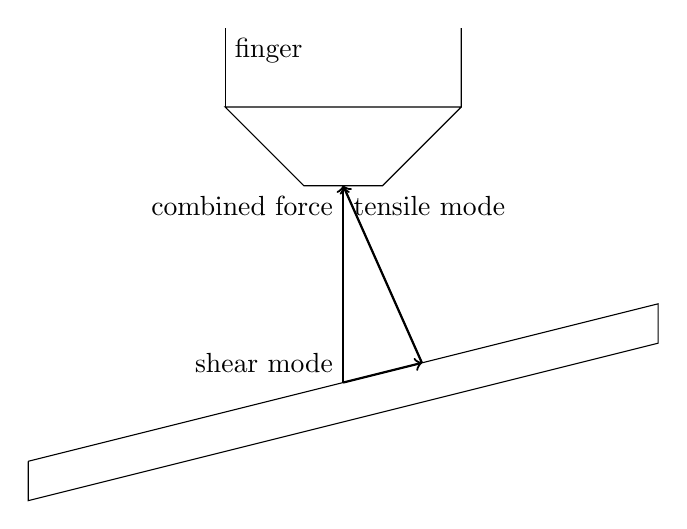
\begin{tikzpicture}
		\draw (-4,0.5) -- (4,2.5) -- (4,2) -- (-4,0) -- (-4,0.5);
		\draw (1.5,5) -- (.5,4) -- (-.5,4) -- (-1.5,5) -- (1.5,5) --(1.5,6);
		\draw (-1.5,5) -- (-1.5,6) node[anchor=north west] {finger};
		\draw[thick, ->] (0,1.5) -- (0,4) node[anchor=north east] {combined force};
		\draw[thick, ->] (0,1.5)  node[anchor=south east] {shear mode} -- (1,1.75);
		\draw[thick, ->] (1,1.75)-- (0,4) node[anchor=north west] {tensile mode};
		
	\end{tikzpicture}
	\caption{Tensile vs Shear mode}
	\label{fig:tensilevsshear}
\end{figure}

\subsection{ice thickness}

\section{PDMS}

Why PDMS was chosen

\subsection{Preparation of PDMS samples}

All PDMS samples with different mixtures are prepared in the same way. The preparation starts with weighting out the needed amount of base coat and curing agent. The mixture is now stirred intensively. Then the mixture is placed in a vacuum bell for 30 minutes to gas out air bubbles. Meanwhile the cover glasses used as slides are cleaned with ethanol or isopropanol. Afterwards, the DPMS mixture is coat-spinned on the cover glass for 5 seconds with 300 rpm and then 120 seconds with 3000 rpm. Then the coated cover glasses are baked in the oven for 30 minutes exept a mixture of 1 base coat and 2 curing agent mixing ratio PDMS. For those 24 hours are needed, as it takes longer to harden and it will result in unwanted effects at plasma curing.

\subsection{Influence of plasma treatment on PDMS}

\subsubsection{setup}

\subsection{detaching ice from PDMS}

1:2 and 4:1

